%!TEX root = ../../book_ML.tex
\chapter{Binary Classifiers cho các bài toán Classification}
 
 
\section{Bài toán phân biệt giới tính dựa trên ảnh khuôn mặt }
Chúng ta cùng bắt đầu với bài toán phân biệt giới tính dựa trên ảnh khuôn mặt. Về ảnh khuôn mặt, bộ cơ sở dữ liệu \href{http://www2.ece.ohio-state.edu/~aleix/ARdatabase.html}{AR Face Database} được sử dụng rộng rãi.  
 
Bộ cơ sở dữ liệu này bao gồm hơn 4000 ảnh màu tương ứng với khuôn mặt của 126 người (70 nam, 56 nữ). Với mỗi người, 26 bức ảnh được chụp ở các điều kiện ánh sáng khác nhau, sắc thái biểu cảm khuôn mặt khác nhau, và bị che mắt (bởi kính râm) hoặc miệng (bởi khăn); và được chụp tại hai thời điểm khác nhau cách nhau 2 tuần.  
 
Để cho đơn giản, tôi sử dụng bộ cơ sử AR Face thu gọn (có thể tìm thấy trong cùng trang web phía trên, mục \textit{Other (relevant) downloads}). Bộ cơ sở dữ liệu thu gọn này bao gồm 2600 bức ảnh từ 50 nam và 50 nữ. Hơn nữa, các khuôn mặt cũng đã được xác định chính xác và được \textit{cropped} với kích thước 165 x 120 (pixel) bằng phương pháp được mô tả trong bài báo \href{http://lectures.molgen.mpg.de/networkanalysis13/PCAversusLDA_eigenfaces.pdf}{PCA veus LDA}. Tôi xin bỏ qua phần xử lý này và trực tiếp sử dụng ảnh đã cropped như một số ví dụ dưới đây: 
 
% <div class="imgcap"> 
% <img src ="\assets\LogReg2\ARgender.png" align = "center" width = "800"> 
% <div class = "thecap">Hình 1: Các ví dụ mẫu trong AR Face database thu gọn.</div> 
% </div>  
\begin{figure}[t]
\centering
    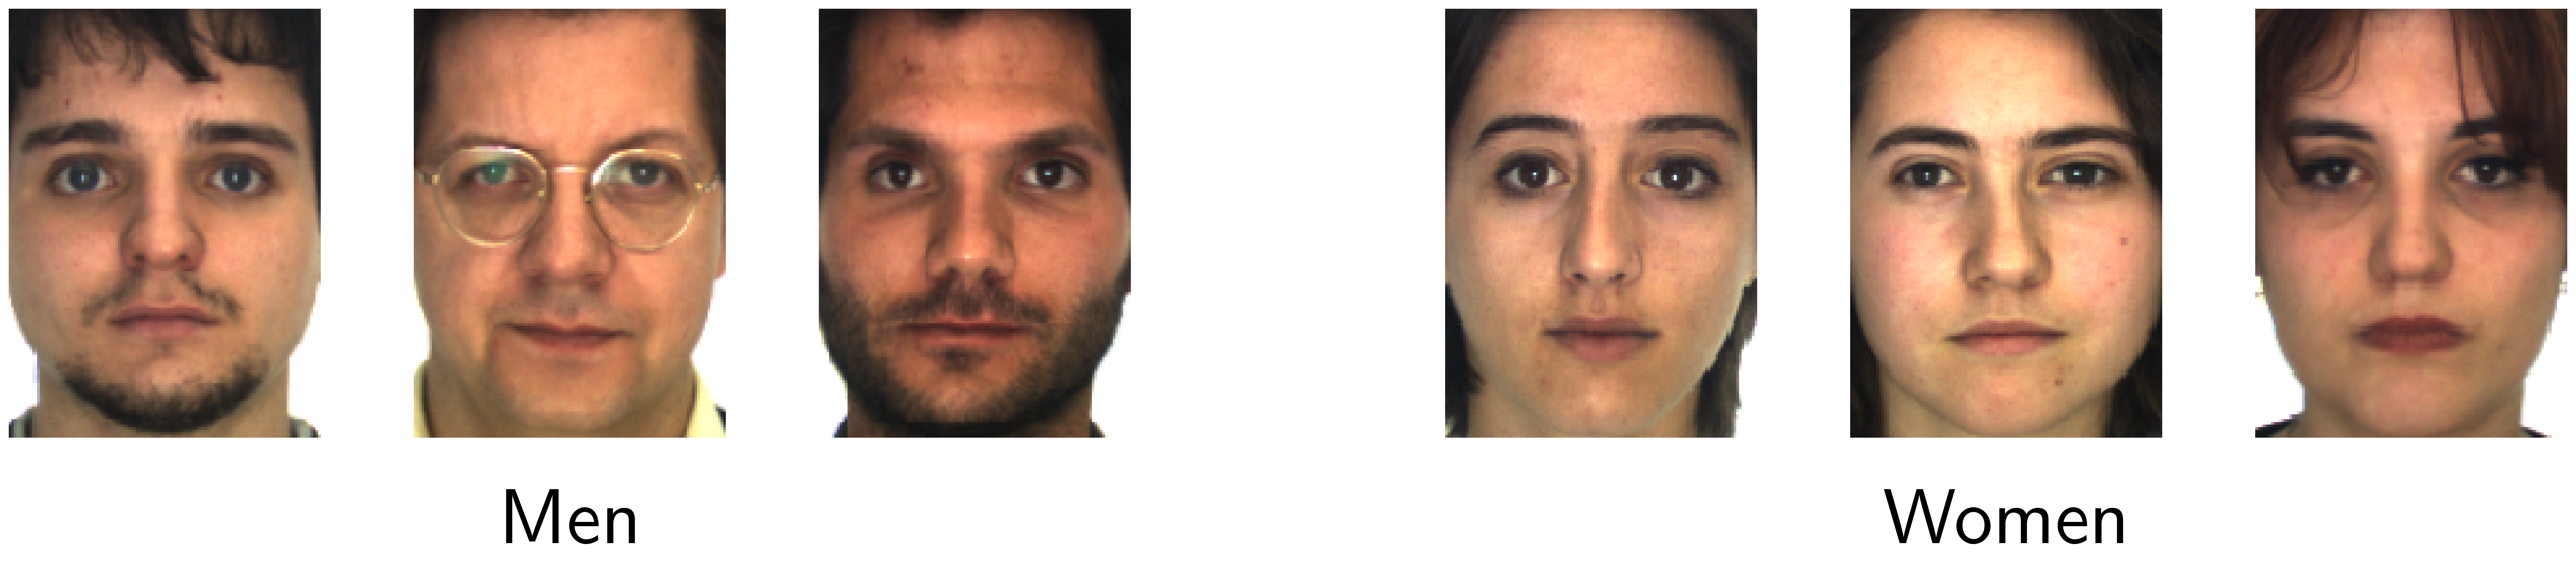
\includegraphics[width = \textwidth]{Chapters/05_NeuralNetworks/12_binaryclassifiers/ARgender.png}
    \caption[]{Các ví dụ mẫu trong AR Face database thu gọn.}
    \label{fig:12_1}
\end{figure}
\textbf{Lưu ý:} 
\begin{itemize}
\item \textit{Vì lý do bản quyền, tôi không được phép chia sẻ với các bạn bộ dữ liệu này. Các bạn muốn sở hữu có thể liên lạc với tác giả như hướng dẫn ở trong website \href{http://www2.ece.ohio-state.edu/~aleix/ARdatabase.html}{AR Face Database}. Một khi các bạn đã có tài khoản để download, tôi mong các bạn tôn trọng tác giả và không chia sẻ trực tiếp với bạn bè.} 
 
\item \textit{Có một cách đơn giản và nhanh hơn để lấy được các feature vector (sau bước \href{http://machinelearningcoban.com/general/2017/02/06/featureengineering/}{Feature Engineering})  của cơ sở dữ liệu này mà không cần liên lạc với tác giả. Các bạn có thể tìm  \href{https://www.umiacs.umd.edu/~zhuolin/projectlcksvd.html}{tại đây}, phần \textbf{Downloads}, mục \textbf{Random face features for AR database}.} 
\end{itemize}
 
Mỗi bức ảnh trong AR Face thu gọn được đặt tên dưới dạng \pythoninline{G-xxx-yy.bmp} Trong đó: \pythoninline{G} nhận một trong hai giá trị \pythoninline{M} (man) hoặc \pythoninline{W} (woman); \pythoninline{xxx} là id của người, nhận gía trị từ \pythoninline{001} đến \pythoninline{050}; \pythoninline{yy} là điều kiện chụp, nhận giá trị từ \pythoninline{01} đến \pythoninline{26}, trong đó các điều kiện có số thứ tự từ \pythoninline{01} đến \pythoninline{07} và từ \pythoninline{14} đến \pythoninline{20} là các khuôn mặt không bị che bởi kính hoặc khăn. Tôi tạm gọi mỗi \textit{điều kiện} này là một \textit{view}. 
 
Để làm ví dụ cho thuật toán Logistic Regression, tôi lấy ảnh của 25 nam và 25 nữ đầu tiên làm tập training set; 25 nam và 25 nữ còn lại làm test set. Với mỗi người, tôi chỉ lấy các khuôn mặt không bị che bởi kính và khăn. 
 
\textbf{Feature Extraction}: vì mỗi bức ảnh có kích thước \pythoninline{3x165x120} (số channels \pythoninline{3}, chiều cao \pythoninline{165}, chiều rộng \pythoninline{120}) là một số khá lớn nên ta sẽ làm thực hiện Feature Extraction bằng hai bước đơn giản sau (\textit{bạn đọc được khuyến khích đọc bài \href{http://machinelearningcoban.com/general/2017/02/06/featureengineering/}{Giới thiệu về Feature Engineering}}):  
\begin{itemize}
    \item Chuyển ảnh màu về ảnh xám theo công thức \pythoninline{Y' = 0.299 R + 0.587 G + 0.114 B } (Xem thêm tại \href{https://en.wikipedia.org/wiki/Grayscale#Luma_coding_in_video_systems}{Grayscale - wiki}).  
     
    \item \textit{Kéo dài} ảnh xám thu được thành 1 vector hàng có số chiều \pythoninline{165x120}, sau đó sử dụng một \textit{random projection matrix} để giảm số chiều về \pythoninline{500}. Bạn đọc có thể thay giá trị này bằng các số khác nhỏ hơn \pythoninline{1000}.  
\end{itemize}
 
Chúng ta có thể bắt đầu làm việc với Python ngay bây giờ. Chúng ta sẽ sử dụng hàm \href{http://scikit-learn.org/stable/modules/generated/sklearn.linear_model.LogisticRegression.html}{\pythoninline{sklearn.linear\_model.LogisticRegression}} trong thư viện \pythoninline{sklearn} cho các ví dụ trong bài này. Nếu không muốn đọc phần này, bạn có thể lấy \href{http://machinelearningcoban.com/assets/LogRegs/ARgender.py}{source code ở dây}.  
 
\textbf{Chú ý:} Hàm \href{http://scikit-learn.org/stable/modules/generated/sklearn.linear_model.LogisticRegression.html}{\pythoninline{sklearn.linear\_model.LogisticRegression}} cũng như các hàm khác của thư viện \pythoninline{sklearn} nhận dữ liệu ở dạng vector hàng, tức mỗi điểm dữ liệu là một hàng trong ma trận dữ liệu. 
 
 
\subsection{Làm việc với Python}
 
Khai báo thư viện 
 
\begin{lstlisting}[language=Python]
import numpy as np  
from sklearn import linear_model           # for logistic regression 
from sklearn.metrics import accuracy_score # for evaluation 
from scipy import misc                     # for loading image 
np.random.seed(1)                          # for fixing random values 
\end{lstlisting}
 
 
Phân chia training set và test set, lựa chọn các \textit{views}. 
 
\begin{lstlisting}[language=Python]
path = '../data/AR/' # path to the database  
train_ids = np.arange(1, 26) 
test_ids = np.arange(26, 50) 
view_ids = np.hstack((np.arange(1, 8), np.arange(14, 21))) 
\end{lstlisting}
 
Tạo \textit{random projection matrix}.  
 
 
\begin{lstlisting}[language=Python]
D = 165*120 # original dimension  
d = 500 # new dimension  
 
# generate the projection matrix  
ProjectionMatrix = np.random.randn(D, d)  
\end{lstlisting}
 
Xây dựng danh sách các tên files. 
 
\begin{lstlisting}[language=Python]
def build_list_fn(pre, img_ids, view_ids): 
    """ 
    INPUT: 
        pre = 'M-' or 'W-' 
        img_ids: indexes of images 
        view_ids: indexes of views 
    OUTPUT: 
        a list of filenames  
    """ 
    list_fn = [] 
    for im_id in img_ids: 
        for v_id in view_ids: 
            fn = path + pre + str(im_id).zfill(3) + '-' + \ 
                str(v_id).zfill(2) + '.bmp' 
            list_fn.append(fn) 
    return list_fn  
\end{lstlisting}
 
\textbf{Feature Extraction:} Xây dựng dữ liệu cho training set và test set. 
 
\begin{lstlisting}[language=Python]
def rgb2gray(rgb): 
#     Y' = 0.299 R + 0.587 G + 0.114 B  
    return rgb[:,:,0]*.299 + rgb[:, :, 1]*.587 + rgb[:, :, 2]*.114 
 
# feature extraction  
def vectorize_img(filename):     
    # load image  
    rgb = misc.imread(filename) 
    # convert to gray scale  
    gray = rgb2gray(rgb) 
    # vectorization each row is a data point  
    im_vec = gray.reshape(1, D) 
    return im_vec  
 
def build_data_matrix(img_ids, view_ids): 
    total_imgs = img_ids.shape[0]*view_ids.shape[0]*2  
         
    X_full = np.zeros((total_imgs, D)) 
    y = np.hstack((np.zeros((total_imgs/2, )), np.ones((total_imgs/2, )))) 
     
    list_fn_m = build_list_fn('M-', img_ids, view_ids) 
    list_fn_w = build_list_fn('W-', img_ids, view_ids) 
    list_fn = list_fn_m + list_fn_w  
     
    for i in range(len(list_fn)): 
        X_full[i, :] = vectorize_img(list_fn[i]) 
 
    X = np.dot(X_full, ProjectionMatrix) 
    return (X, y) 
 
(X_train_full, y_train) = build_data_matrix(train_ids, view_ids) 
x_mean = X_train_full.mean(axis = 0) 
x_var  = X_train_full.var(axis = 0) 
 
def feature_extraction(X): 
    return (X - x_mean)/x_var      
 
X_train = feature_extraction(X_train_full) 
X_train_full = None ## free this variable  
 
(X_test_full, y_test) = build_data_matrix(test_ids, view_ids) 
X_test = feature_extraction(X_test_full) 
X_test_full = None  
\end{lstlisting}
 
\textbf{Chú ý:} Trong đoạn code trên tôi có sử dụng phương pháp chuẩn hóa dữ liệu \href{http://machinelearningcoban.com/general/2017/02/06/featureengineering/#standardization}{Standardization}. Trong đó \pythoninline{x_mean} và \pythoninline{x_var} lần lượt là vector kỳ vọng và phương sai của toàn bộ dữ liệu training. \pythoninline{X_train_full}, \pythoninline{X_test_full} là các ma trận dữ liệu đã được giảm số chiều nhưng chưa được chuẩn hóa. Hàm \pythoninline{feature_extraction} giúp chuẩn hóa dữ liệu dựa vào \pythoninline{x_mean} và \pythoninline{x_var} của \pythoninline{X_train_full}. 
 
Đoạn code dưới đây thực hiện thuật toán Logistic Regression, dự đoán output của test data và đánh giá kết quả. Một chú ý nhỏ, hàm Logistic Regression trong thư viện sklearn có nhiều biến thể khác nhau. Để sử dụng thuật toán Logistic Regression \textit{thuần} mà tôi đã giới thiệu trong bài \href{http://machinelearningcoban.com/2017/01/27/logisticregression/}{Logistic Regression}, chúng ta cần đặt giá trị cho \pythoninline{C} là một số lớn (để nghịch đảo của nó gần với 0. Tạm thời các bạn chưa cần quan tâm tới điều này, chỉ cần chọn \pythoninline{C} lớn là được). 
 
 
\begin{lstlisting}[language=Python]
logreg = linear_model.LogisticRegression(C=1e5) # just a big number  
logreg.fit(X_train, y_train) 
 
y_pred = logreg.predict(X_test) 
print "Accuracy: %.2f %%" %(100*accuracy_score(y_test, y_pred)) 
\end{lstlisting}
Kết quả:
\begin{lstlisting}
    Accuracy: 90.33 % 
\end{lstlisting}
 
90.33\%, tức là cứ 10 bức ảnh trong test set thì có trung bình hơn 9 bức được nhận dạng đúng. Không tệ, nhất là khi chúng ta vẫn chưa phải làm gì nhiều! 
 
Để xác định \textit{nhãn} của một ảnh, đầu ra của hàm \href{http://machinelearningcoban.com/2017/01/27/logisticregression/#sigmoid-function}{sigmoid} được so sánh với 0.5. Nếu giá trị đó lớn hơn 0.5, ta kết luận đó là ảnh của nam, ngược lại, đó là ảnh của nữ. Để xem giá trị sau hàm sigmoid (tức xác suất để ảnh đó là nam), chúng ta sử dụng hàm \pythoninline{predict_proba} như sau: 
 
\begin{lstlisting}[language=Python]
def feature_extraction_fn(fn): 
    """ 
    extract feature from filename 
    """ 
    # vectorize 
    im = vectorize_img(fn) 
    # project 
    im1 = np.dot(im, ProjectionMatrix) 
    # standardization  
    return feature_extraction(im1) 
 
fn1 = path + 'M-036-18.bmp' 
fn2 = path + 'W-045-01.bmp' 
fn3 = path + 'M-048-01.bmp' 
fn4 = path + 'W-027-02.bmp' 
 
x1 = feature_extraction_fn(fn1) 
p1 = logreg.predict_proba(x1) 
print(p1) 
 
x2 = feature_extraction_fn(fn2) 
p2 = logreg.predict_proba(x2) 
print(p2) 
 
x3 = feature_extraction_fn(fn3) 
p3 = logreg.predict_proba(x3) 
print(p3) 
 
x4 = feature_extraction_fn(fn4) 
p4 = logreg.predict_proba(x4) 
print(p4) 
\end{lstlisting}
\begin{lstlisting}
    [[ 0.87940218  0.12059782]] 
    [[ 0.0172217  0.9827783]] 
    [[ 0.30458761  0.69541239]] 
    [[ 0.83989242  0.16010758]] 
\end{lstlisting}
 
Kết quả thu được là xác suất để bức ảnh đó là ảnh của nam (cột thứ nhất) và của nữ (cột thứ hai). Dưới đây là hình minh họa: 
 
% <div class="imgcap"> 
% <img src ="\assets\LogReg2\ARgenderResult.png" align = "center" width = "800"> 
% <div class = "thecap">Hình 2: Ví dụ về kết quả tìm được bằng Logistic Regression</div> 
% </div>  
\begin{figure}[t]
 \centering
     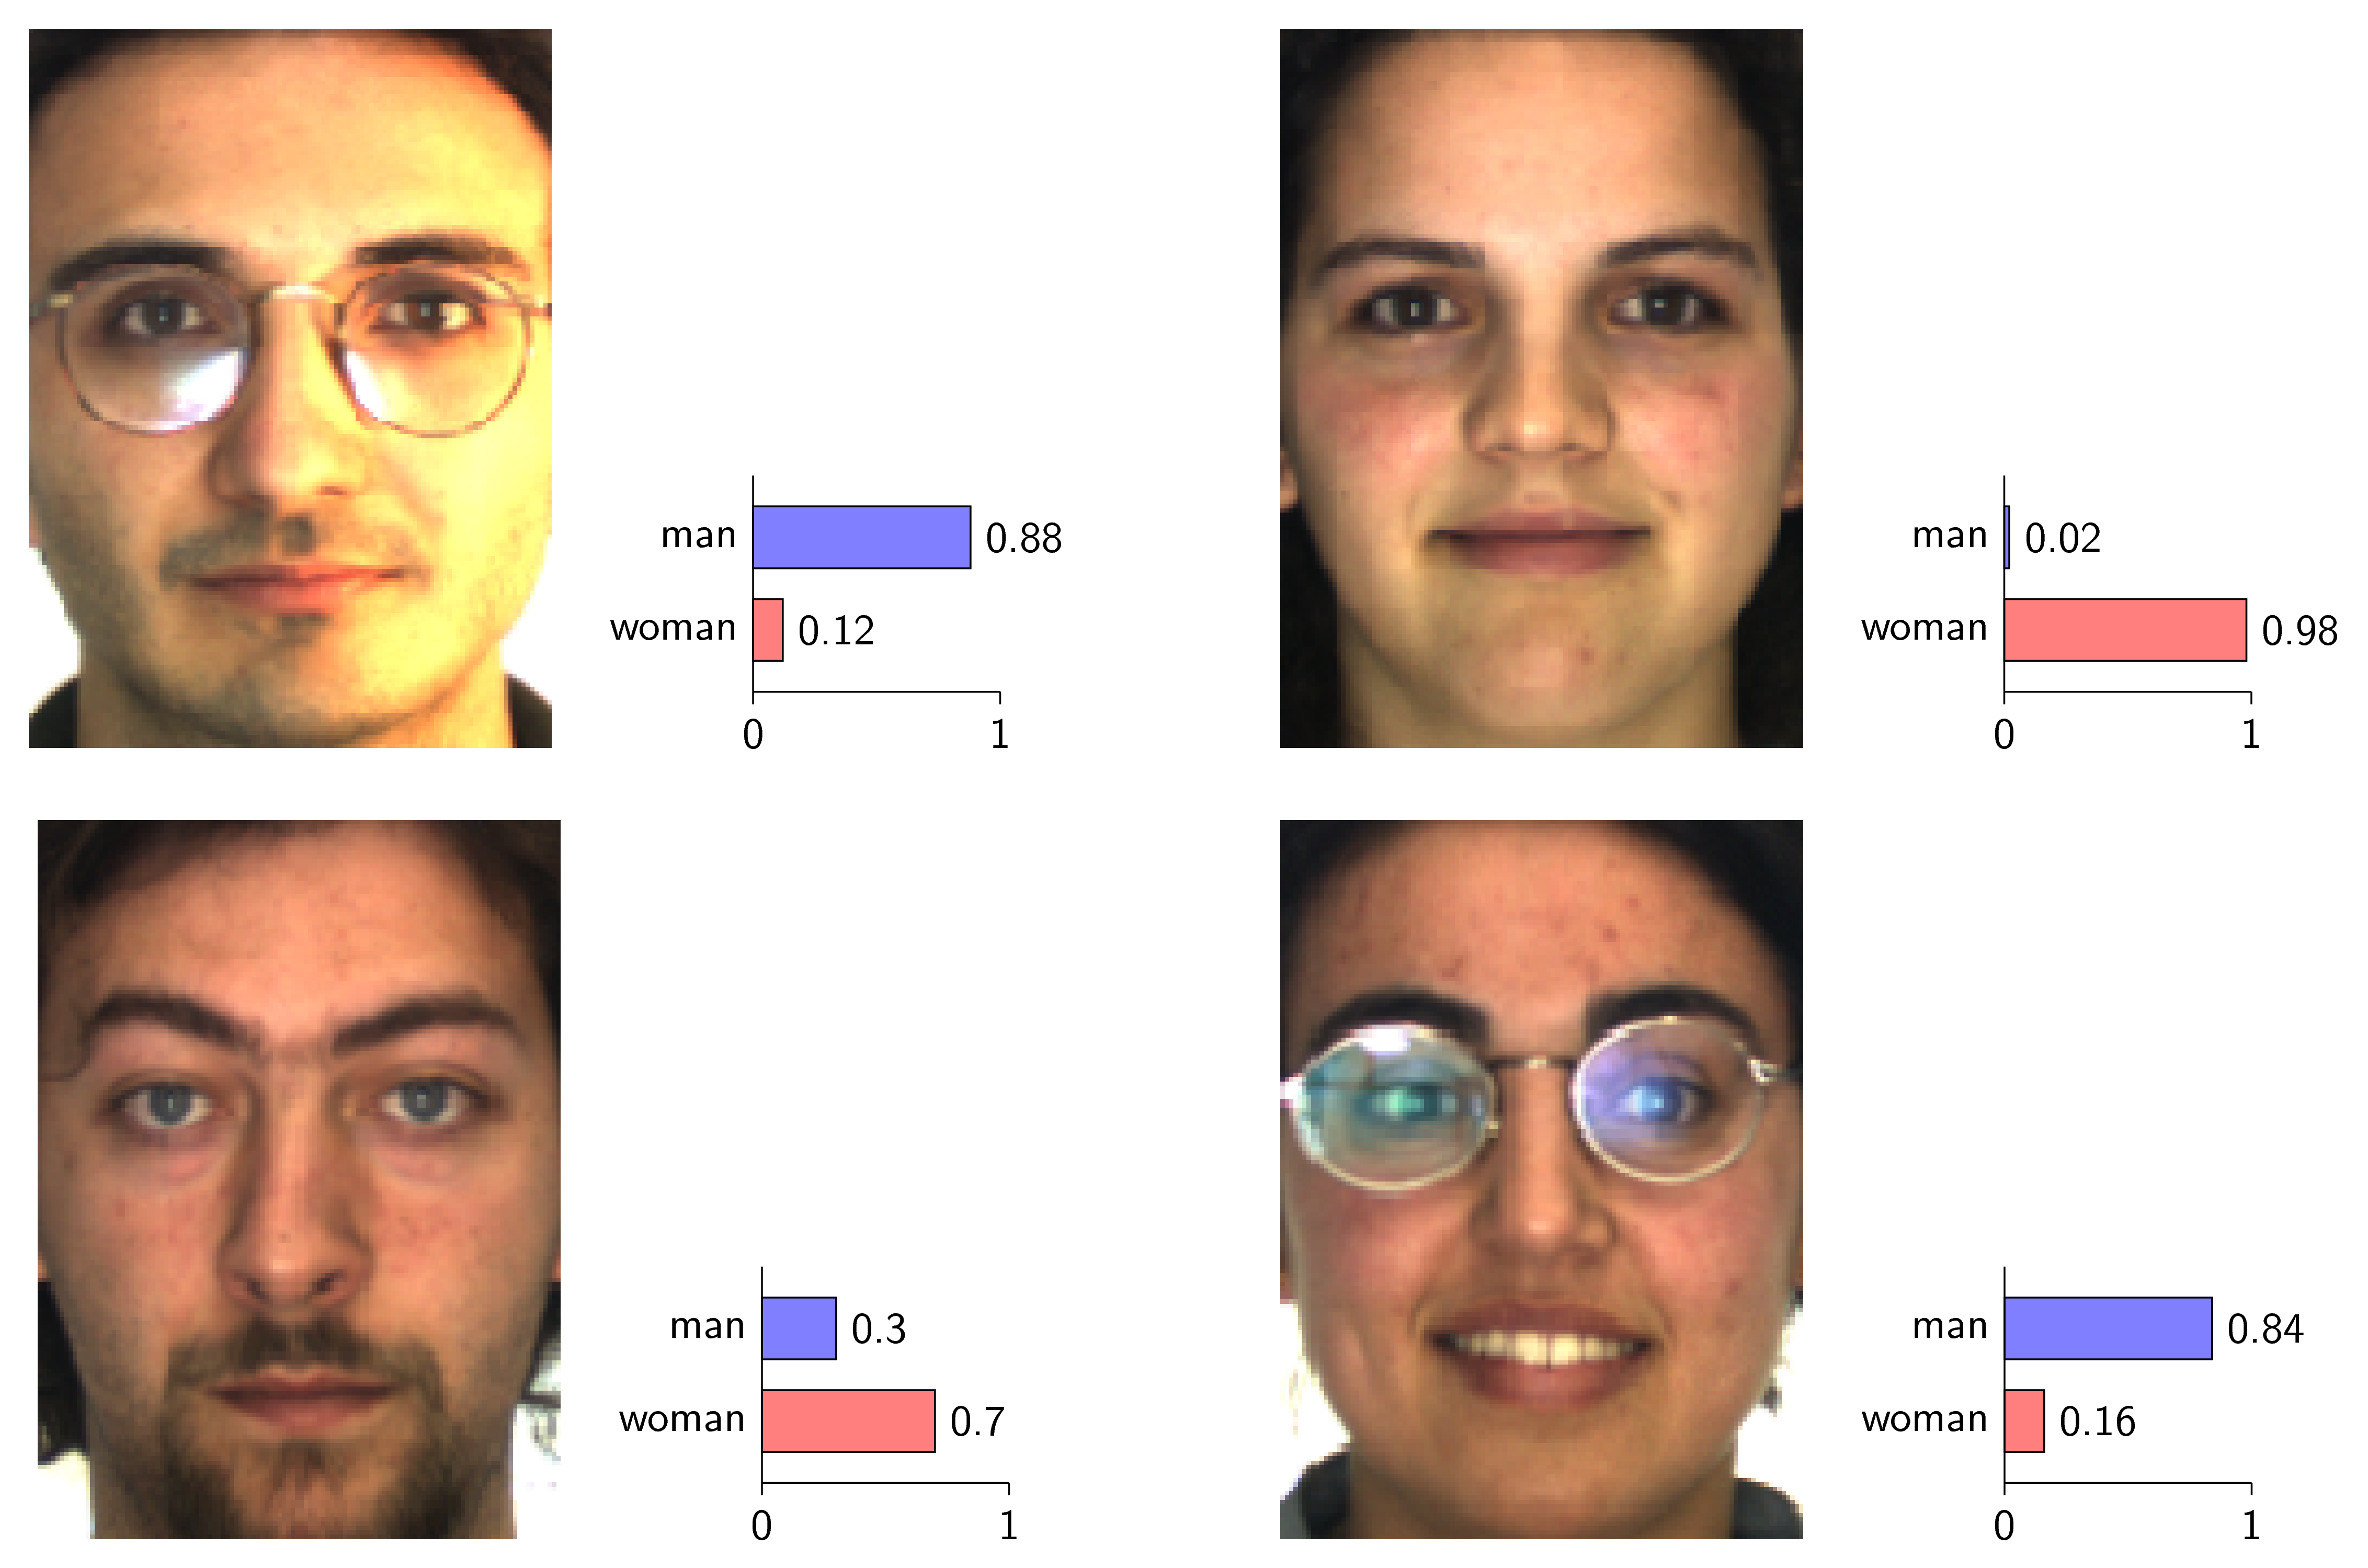
\includegraphics[width = \textwidth]{Chapters/05_NeuralNetworks/12_binaryclassifiers/ARgenderResult.png}
     \caption[]{Ví dụ về kết quả tìm được bằng Logistic Regression.}
     \label{fig:12_2}
 \end{figure} 
Hàng trên gồm các hình được phân loại đúng, hàng dưới gồm các hình bị phân loại sai. Có một vài nhận xét về hàng dưới. Từ hai bức ảnh hàng dưới, chúng ta có thể đoán rằng Logistic Regression quan tâm đến tóc phía sau gáy nhiều hơn là râu! Việc thuật toán dựa trên những đặc trưng nào của mỗi class phụ thuộc rất nhiều vào training data. Nếu trong training data, hầu hết nam không có râu và hầu hết nữ có tóc dài thì kết quả này là có thể lý giải được.  
 
\textbf{Trong Machine Learning, thuật toán là quan trọng, nhưng thuật toán tốt mà dữ liệu không tốt thì sẽ dẫn đến những tác dụng ngược!} 
 
(Source code cho ví dụ này có thể tìm thấy \href{https://github.com/tiepvupsu/tiepvupsu.github.io/blob/master/assets/LogReg2/ARGender.ipynb}{ở dây}.) 
 
\section{Bài toán phân biệt hai chữ số viết tay }
Chúng ta cùng sang ví dụ thứ hai về phân biệt hai chữ số trong \href{http://machinelearningcoban.com/2017/01/04/kmeans2/#bo-co-so-du-lieu-mnist}{bộ cơ sở dữ liệu MNIST}. Cụ thể, tôi sẽ làm việc với hai chữ số 0 và 1. Bạn đọc hoàn toàn có thể thử với các chữ số khác bằng cách thay đổi một dòng lệnh. Khác với AR Face, bộ dữ liệu này có thể dễ dàng được download về từ \href{http://yann.lecun.com/exdb/mnist/}{trang chủ} của nó. 
 
Chúng ta có thể bắt tay vào làm luôn.  
 
Khai báo thư viện: 
 
\begin{lstlisting}[language=Python]
# %reset 
import numpy as np  
from mnist import MNIST 
import matplotlib.pyplot as plt 
from sklearn import linear_model 
from sklearn.metrics import accuracy_score 
from display_network import * 
\end{lstlisting}
 
Load toàn bộ dữ liệu: 
 
\begin{lstlisting}[language=Python]
mntrain = MNIST('../MNIST/') 
mntrain.load_training() 
Xtrain_all = np.asarray(mntrain.train_images) 
ytrain_all = np.array(mntrain.train_labels.tolist()) 
 
mntest = MNIST('../MNIST/') 
mntest.load_testing() 
Xtest_all = np.asarray(mntest.test_images) 
ytest_all = np.array(mntest.test_labels.tolist()) 
\end{lstlisting}
 
Sau bưóc này, toàn bộ dữ liệu training data và test data được lưu ở hai ma trận \pythoninline{X_train_all} và \pythoninline{X_test_all}, mỗi hàng của các ma trận này chứa một điểm dữ liệu, tức một bức ảnh đã được \textit{vector hóa}.  
 
Để lấy các hàng tương ứng với chữ số 0 và chữ số 1, ta khai báo biến sau: 
 
\begin{lstlisting}[language=Python]
cls = [[0], [1]] 
\end{lstlisting}
 
Nếu bạn muốn thử với cặp \pythoninline{3} và \pythoninline{4}, chỉ cần thay dòng này bằng \pythoninline{cls = [[3], [4]]}. Nếu bạn muốn phân loại \pythoninline{(4, 7)} và \pythoninline{(5, 6)}, chỉ cần thay dòng này bằng \pythoninline{cls = [[4, 7], [5, 6]]}. Các cặp bất kỳ khác đều có thể thực hiện bằng cách thay chỉ một dòng này.  
 
Đoạn code dưới đây thực hiện việc \textit{extract} toàn bộ dữ liệu cho các chữ số \pythoninline{0} và \pythoninline{1} trong tập training data và test data.  
 
\begin{lstlisting}[language=Python]
def extract_data(X, y, classes): 
    """ 
    X: numpy array, matrix of size (N, d), d is data dim 
    y: numpy array, size (N, ) 
    cls: two lists of labels. For example:  
        cls = [[1, 4, 7], [5, 6, 8]] 
    return: 
        X: extracted data 
        y: extracted label  
            (0 and 1, corresponding to two lists in cls) 
    """ 
    y_res_id = np.array([]) 
    for i in cls[0]: 
        y_res_id = np.hstack((y_res_id, np.where(y == i)[0])) 
    n0 = len(y_res_id) 
 
    for i in cls[1]: 
        y_res_id = np.hstack((y_res_id, np.where(y == i)[0])) 
    n1 = len(y_res_id) - n0  
 
    y_res_id = y_res_id.astype(int) 
    X_res = X[y_res_id, :]/255.0 
    y_res = np.asarray([0]*n0 + [1]*n1) 
    return (X_res, y_res) 
 
 
# extract data for training  
(X_train, y_train) = extract_data(Xtrain_all, ytrain_all, cls) 
 
# extract data for test  
(X_test, y_test) = extract_data(Xtest_all, ytest_all, cls) 
\end{lstlisting}
 
Vì mỗi điểm dữ liệu có số phần tử là 784 (28x28), là một số khá nhỏ, nên ta không cần thêm bước giảm số chiều dữ liệu nữa. Tuy nhiên, tôi có thực hiện thêm một bước chuẩn hóa để đưa dữ liệu về đoạn \pythoninline{[0, 1]} bằng cách chia toàn bộ hai ma trận dữ liệu cho \pythoninline{255.0}. 
 
Tới đây ta có thể \textit{train} mô hình Logistic Regression và đánh giá mô hình này.   
 
\begin{lstlisting}[language=Python]
# train the logistic regression model  
logreg = linear_model.LogisticRegression(C=1e5) # just a big number  
logreg.fit(X_train, y_train) 
 
# predict  
y_pred = logreg.predict(X_test) 
print "Accuracy: %.2f %%" %(100*accuracy_score(y_test, y_pred.tolist())) 
\end{lstlisting}
Kết quả:
\begin{lstlisting}
    Accuracy: 99.95 % 
\end{lstlisting}
 
Tuyệt vời, gần như 100\% được phân loại chính xác. Điều này là dễ hiểu vì hai chữ số 0 và 1 khác nhau quá nhiều. Bộ cơ sở dữ liệu này với toàn bộ 10 classes hiện nay đã được phân loại với độ chính xác trên 99.7\%.  
 
Chúng ta cùng đi tìm những ảnh bị phân loại sai: 
 
\begin{lstlisting}[language=Python]
# display misclassified image(s) 
mis = np.where((y_pred - y_test) != 0)[0] 
Xmis = X_test[mis, :] 
 
plt.axis('off') 
A = display_network(Xmis.T) 
f2 = plt.imshow(A, interpolation='nearest' ) 
plt.gray() 
plt.show() 
\end{lstlisting}
 
% <div class="imgcap"> 
% <img src ="\assets\LogReg2\0.png" align = "center" width = "100"> 
% <div class = "thecap">Hình 3: Chữ số bị phân loại sai trong bài toán phân loại ảnh chữ số 0 và 1</div> 
% </div>  
\begin{figure}[t]
    % caption on side     
    \floatbox[{\capbeside\thisfloatsetup{capbesideposition={right,top},capbesidewidth=12cm}}]{figure}[\FBwidth]
    {\caption{ 
    Chữ số bị phân loại sai trong bài toán phân loại ảnh chữ số 0 và 1.
    }
    \label{fig:10_3}}
    { % figure here
    
\includegraphics[width=.15\textwidth]{Chapters/05_NeuralNetworks/12_binaryclassifiers/0.png}
    }
\end{figure}

Như vậy là chỉ có một ảnh bị phân loại sai. Ảnh này là chữ số 0 nhưng bị misclassified thành chữ số 1, có thể vì nét đậm nhất của nó rất giống với chữ số 1.  
 
Source code cho ví dụ này có thể được tìm thấy \href{http://machinelearningcoban.com/assets/LogReg2/LogReg2.ipynb}{ở đây}. 
 
 
\section{Binary Classifiers cho Multi-class Classification problems }
 
Có lẽ nhiều bạn đang đặt câu hỏi: Các ví dụ trên đây đều làm với bài toán có hai classes. Vậy nếu có nhiều hơn hai classes, ví dụ như 10 classes của MNIST, thì làm thế nào? 
 
Có nhiều thuật toán khác được xây dựng riêng cho các bài toán với nhiều classes (multi-class classification problems), tôi sẽ giới thiệu sau. Còn bây giờ, chúng ta vẫn có thể sử dụng các \textit{binary classifiers} để thực hiện công việc này, với một chút thay đổi.  
 
Có \textit{ít nhất} bốn cách để áp dụng \textit{binary classifiers} vào các bài toán multi-class classification: 
 
 
\subsection{One-vs-one}
 
Xây dựng rất nhiều bộ binary classifiers cho từng cặp classes. Bộ thứ nhất phân biệt class 1 và class 2, bộ thứ hai phân biệt class 1 và class 3, ... Khi có một dữ liệu mới vào, đưa nó vào toàn bộ các bộ binary classifiers trên. Kết quả cuối cùng có thể được xác định bằng cách xem class nào mà điểm dữ liệu đó được phân vào nhiều nhất (major voting). Hoặc với Logistic Regression thì ta có thể tính \textit{tổng các xác suất} tìm được sau mỗi bộ binary classifier.  
  
Như vậy, nếu có $C$ classes thì tổng số binary classifiers phải dùng là $\frac{n(n-1)}{2}$. Đây là một con số lớn, cách làm này không lợi về tính toán. Hơn nữa, nếu một chữ số thực ra là chữ số \pythoninline{1}, nhưng lại được đưa vào bộ phân lớp giữa các chữ số \pythoninline{5} và \pythoninline{6}, thì cả hai khả năng tìm được (là \pythoninline{5} hoặc \pythoninline{6}) đều không hợp lý! 
 
 
\subsection{Hierarchical (phân tầng)}
Các làm như \textbf{one-vs-one} sẽ mất rất nhiều thời gian training vì có quá nhiều bộ phân lớp cần được xây dựng. Một cách khác giúp \textit{tiết kiệm} số binary classifiers hơn đó là \textbf{hierarchical}. Ý tưởng như sau: 
 
Ví dụ với MNIST với 4 chữ số \pythoninline{4, 5, 6, 7}. Vì ta thấy chữ số \pythoninline{4} và \pythoninline{7} khá giống nhau, chữ số \pythoninline{5} và \pythoninline{6} khá giống nhau nên trước tiên chúng ta xây dựng bộ phân lớp \pythoninline{[4, 7] vs [5, 6]}. Sau đó xây dựng thêm hai bộ \pythoninline{4 vs  7} và \pythoninline{5 vs 6} nữa. Tổng cộng, ta cần 3 bộ binary classifiers. Chú ý rằng có nhiều cách chia khác nhau, ví dụ \pythoninline{[4, 5, 6] vs 7}, \pythoninline{[4, 5] vs 6}, rồi \pythoninline{4 vs 5}.  
 
 
Ưu điểm của phương pháp này là sử dụng ít bộ binary classifiers hơn \textbf{one-vs-one}.  
Hạn chế lớn nhất của nó là việc nếu chỉ một binary classifier cho kết quả sai thì kết quả cuối cùng chắc chắn sẽ sai. Ví dụ, nếu 1 ảnh chứa chữ số \pythoninline{5}, nhưng ngay bước đầu tiên đã bị misclassifed sang nhánh \pythoninline{[4, 7]} thì kết quả cuối cùng sẽ là \pythoninline{4} hoặc \pythoninline{7}, cả hai đều sai.  
 
 
\subsection{Binary coding}
Có một cách giảm số binary classifiers hơn nữa là \textbf{binary coding}, tức \textit{mã hóa} output của mỗi class bằng một số nhị phân. Ví dụ, nếu có 4 classes thì class thứ nhất được mã hóa là \pythoninline{00}, ba class kia được mã hóa lần lượt là \pythoninline{01, 10} và \pythoninline{11}. Với cách làm này, số bộ binary classifiers phải thực hiện chỉ là $m = \left\lceil\log_2(C)\right\rceil$ trong đó $C$ là số lượng class, $\left\lceil a \right\rceil$ là \textit{số nguyên nhỏ nhất không nhỏ hơn} $a$. Class thứ nhất sẽ đi tìm bit đầu tiên của output (đã được mã hóa nhị phân), class thứ hai sẽ đi tìm bit thứ hai, ... 
 
Cách làm này sử dụng một số lượng nhỏ nhất các bộ \textit{binary classifiers}. Nhưng nó có một hạn chế rất lớn là chỉ cần một bit bị phân loại sai sẽ dẫn đến dữ liệu bị phân loại sai. Hơn nữa, nếu số classes không phải là lũy thừa của hai, mã nhị phân nhận được có thể là một giá trị không tương ứng với class nào! 
 
 
\subsection{one-vs-rest hay one-hot coding}
Phương pháp được sử dụng nhiều nhất là \textbf{one-vs-rest} (một số tài liệu gọi là \textbf{ove-vs-all}, \textbf{one-against-rest}, hoặc \textbf{one-against-all}) . Cụ thể, nếu có $C$ classes thì ta sẽ xây dựng $C$ classifiers, mỗi classifier tương ứng với một class. Classifier thứ nhất giúp phân biệt \pythoninline{class 1} vs \pythoninline{not class 1}, tức xem một điểm có thuộc class 1 hay không, hoặc xác suất để một điểm rơi vào class 1 là bao nhiêu. Tương tự như thế, classifier thứ hai sẽ phân biệt \pythoninline{class 2} vs \pythoninline{not class 2}, ... Kết quả cuối cùng có thể được xác định bằng cách xác định class mà một điểm rơi vào với xác suất cao nhất.  
 
Phương pháp này còn được gọi là \textbf{one-hot coding} (được sử dụng nhiều nên có rất nhiều tên) vì với cách mã hóa trên, giả sử có 4 classes, class 1, 2, 3, 4 sẽ lần lượt được mã hóa dưới dạng nhị phân bởi \pythoninline{1000, 0100, 0010} hoặc \pythoninline{0001}. One-hot vì chỉ có \textit{one} bit là \textit{hot} (bằng \pythoninline{1}).  
 
Hàm Logistic Regression trong thư viện sklearn có thể được dùng trực tiếp để áp dụng vào các bài toán multi-class classification với phương pháp \textbf{one-vs-rest}. Với bài toán MNIST như nêu ở phần 2, ta có thể thêm ba dòng lệnh sau để chạy trên toàn bộ 10 classes: 
 
\begin{lstlisting}[language=Python]
logreg.fit(Xtrain_all, ytrain_all) 
y_pred = logreg.predict(Xtest_all) 
print "Accuracy: %.2f %%" %(100*accuracy_score(ytest_all, y_pred.tolist())) 
\end{lstlisting}
 
Kết quả thu được khoảng 91\% sau hơn 20 phút chạy (thời gian chạy này tùy thuộc vào máy). Đây vẫn là một kết quả quá thấp so với con số 99.7\%. Thậm chí phương pháp học máy \textit{không học gì} như \href{http://machinelearningcoban.com/2017/01/08/knn/#try-this-yourself}{K-neareast neighbors cũng đã đạt hơn 96\%} với thời gian chạy ngắn hơn một chút.  
 
Một chú ý nhỏ: phương pháp mặc định cho các bài toán multi-class của hàm này được xác định bởi biến \pythoninline{multi_class}. Có hai lựa chọn cho biến này, trong đó lựa chọn mặc định là \pythoninline{ovr} tức \textbf{one-vs-rest}, lựa chọn còn lại sẽ được tôi đề cập trong một bài gần đây. Lựa chọn thứ hai không phải cho binary classifiers nên tôi không đề cập trong bài này, có thể sau một vài bài nữa (Xem thêm \href{http://scikit-learn.org/stable/modules/generated/sklearn.linear_model.LogisticRegression.html}{\pythoninline{sklearn.linear_model.LogisticRegression}}) 
 
 
 
\section{Thảo luận }
 
\subsection{Kết hợp các phương pháp trên}
 
Nhắc lại rằng các linear binary classifiers tôi đã trình bày yêu cầu dữ liệu là \textit{linearly separable} hoặc \textit{nearly linearly separable}. Ta cũng có thể mở rộng định nghĩa này cho các bài toán multi-class. Nếu hai class bất kỳ là \textit{linearly separable} thì ta coi dữ liệu đó là \textit{linearly separable}.  
 
Thế nhưng, có những loại dữ liệu \textit{linearly separable} mà chỉ một số trong 4 phương pháp trên đây là phù hợp, hoặc có những loại dữ liệu yêu cầu phải kết hợp nhiều phương pháp mới thực hiện được. Xét ba ví dụ trong Hình \eqref{fig:10_4}.
 
% <div class="imgcap"> 
% <img src ="\assets\LogReg2\dist.png" align = "center" width = "800"> 
% <div class = "thecap">Hình 4: Một số ví dụ về phân phối của các classes trong bài toàn multi-class</div> 
% </div>  
\begin{figure}[t]
\centering
    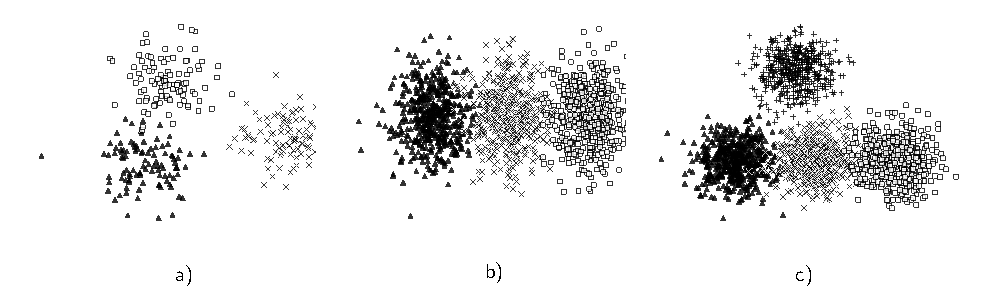
\includegraphics[width = \textwidth]{Chapters/05_NeuralNetworks/12_binaryclassifiers/latex/dist.pdf}
    \caption[]{Một số ví dụ về phân phối của các classes trong bài toán multi-class classification.}
    \label{fig:10_4}
\end{figure}
\begin{itemize}
\item Hình \eqref{fig:10_4}a): cả 4 phương pháp trên đây đều có thể áp dụng được. 
 
\item Hình \eqref{fig:10_4}b): one-vs-rest không phù hợp vì class màu xanh lục và class \textit{rest} (hợp của xanh lam và đỏ) là không \textit{linearly separable}. Lúc này, one-vs-one hoặc hierarchical phù hợp hơn.  
 
\item Hình 4c): Tương tự như trên, ba class lam, lục, đỏ thẳng hàng nên sẽ không dùng được one-vs-rét. one-vs-one vẫn làm việc vì từng đôi class một là \textit{linearly separable}. Tương tự hierarchical cũng làm việc nếu ta phân chia các nhóm một cách hợp lý. Hoặc chúng ta có thể kết hợp nhiều phương pháp. Ví dụ: dùng one-vs-rest để tìm \textit{đỏ} vs \textit{không đỏ}. Nếu một điểm dữ liệu là \textit{không đỏ}, với 3 class còn lại, chúng ta lại quay lại trường hợp Hình 4a) và có thể dùng các phương pháp khác. Nhưng khó khăn vẫn nằm ở việc phân nhóm như thế nào, liệu rằng những class nào có thể cho vào cùng một nhóm? Với những dữ liệu đơn giản, \href{http://machinelearningcoban.com/2017/01/01/kmeans/}{K-means clustering} có thể là một giải pháp! 
\end{itemize}
 
Bạn đọc có thể xem thêm ví dụ áp dụng Logistic Regression cho cơ sở dữ liệu \href{http://machinelearningcoban.com/2017/01/08/knn/#bo-co-so-du-lieu-iris-iris-flower-dataset}{Iris} trong \href{http://scikit-learn.org/stable/auto_examples/linear_model/plot_iris_logistic.html}{link này} 
 
 
 
% <div class="imgcap"> 
% <img src ="http://scikit-learn.org/stable/_images/sphx_glr_plot_iris_logistic_001.png" align = "center" width = "500"> 
% <div class = "thecap">Hình 5: Logistic Regression với Iris database. (Nguồn: <a href="http://scikit-learn.org/stable/auto_examples/linear_model/plot_iris_logistic.html">Logistic Regression 3-class Classifier</a>)</div> 
% </div>  
 
 
 
\subsection{Biểu diễn dưới dạng Neural Networks}
Lấy ví dụ với bài toán có 4 classes 1, 2, 3, 4; ta có thể biểu diễn các mô hình được đề cập trong Mục 3 dưới dạng sau đây (giả sử input có số chiều là 7 và node output màu đỏ biểu diễn chung cho cả PLA, Logistic Regression và các networks với activation function khác) như trong Hình \ref{fig:12_6}.
 
% <div class="imgcap"> 
% <img src ="\assets\LogReg2\binaryclassifiers.png" align = "center" width = "800"> 
% <div class = "thecap">Hình 6: Mô hình neural networks cho các phương pháp đề cập trong bài</div> 
% </div>  
% \begin{figure}[t]
% \centering
%     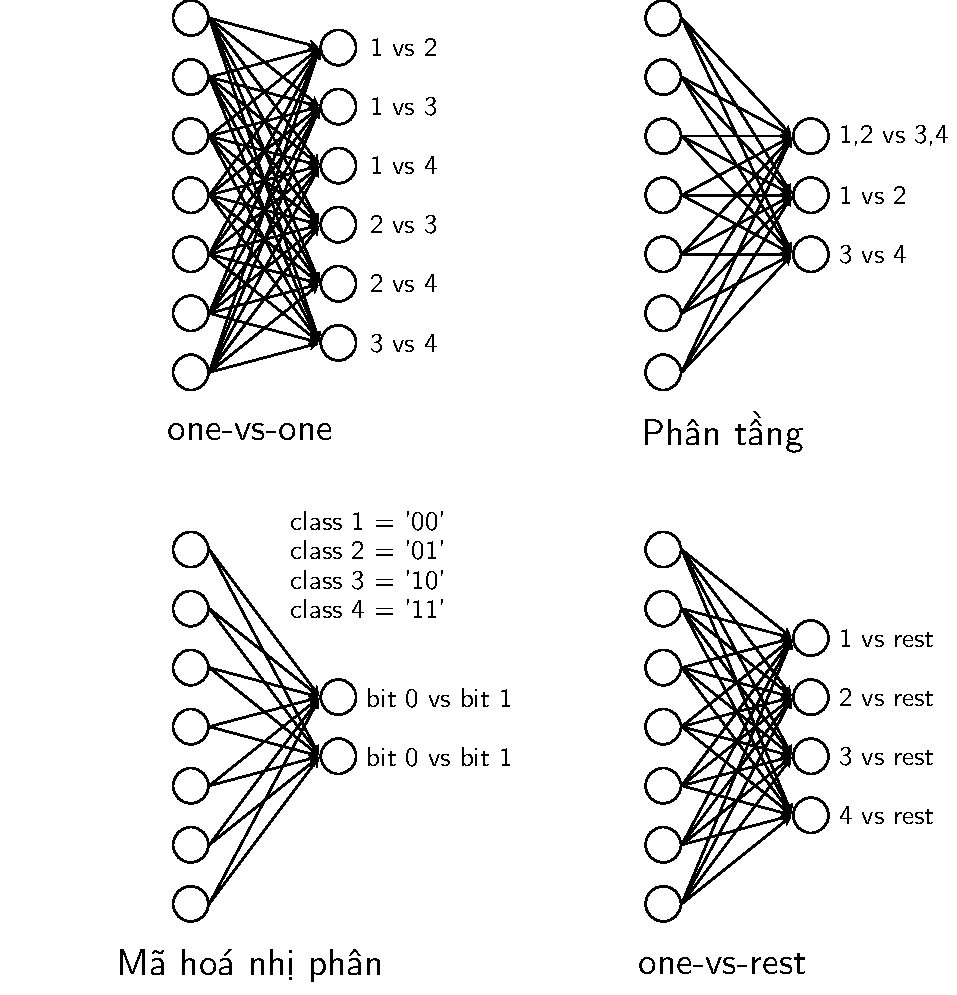
\includegraphics[width = \textwidth]{Chapters/05_NeuralNetworks/12_binaryclassifiers/latex/binaryclassifiers.pdf}
%     \caption[]{Mô hình neural networks cho các phương pháp đề cập trong bài.}
%     \label{fig:12_6}
% \end{figure}

\begin{figure}[t]
    % caption on side     
    \floatbox[{\capbeside\thisfloatsetup{capbesideposition={right,top},capbesidewidth=3cm}}]{figure}[\FBwidth]
    {\caption{ 
    Mô hình neural networks cho các phương pháp đề cập trong bài.
    }
    \label{fig:12_6}}
    { % figure here
    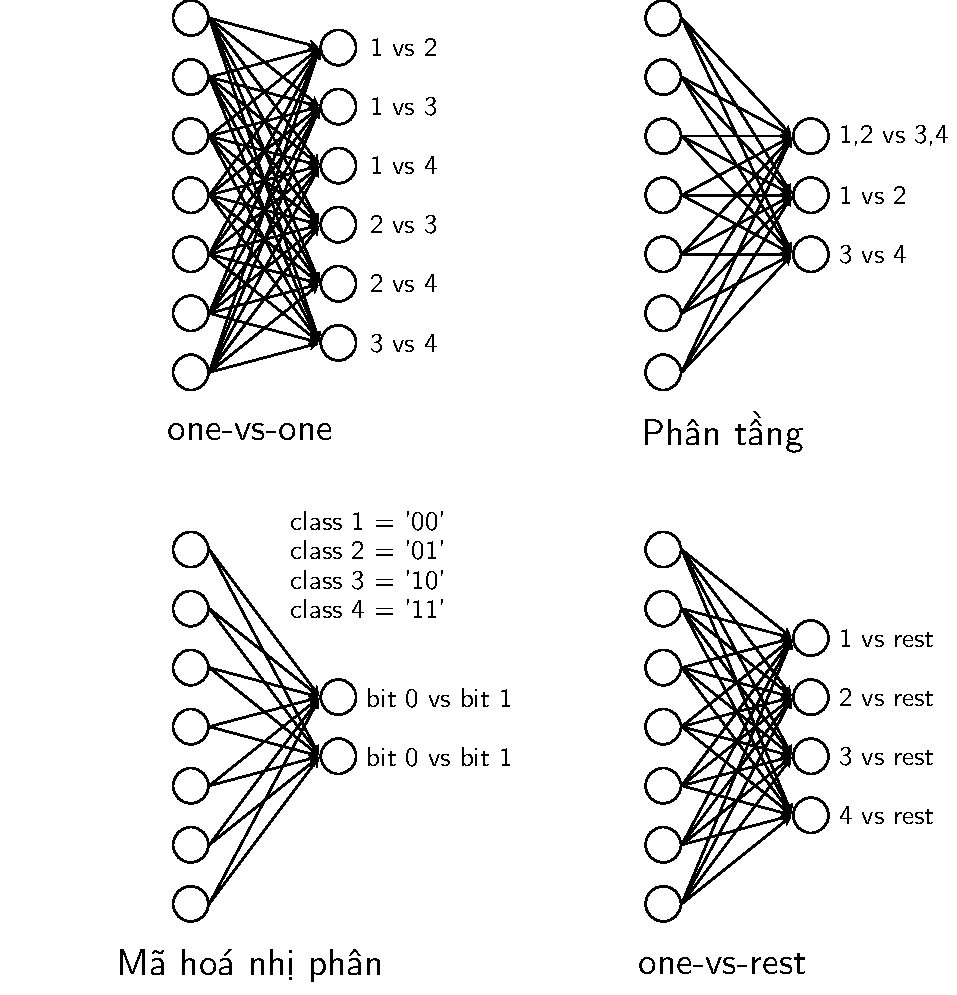
\includegraphics[width=.75\textwidth]{Chapters/05_NeuralNetworks/12_binaryclassifiers/latex/binaryclassifiers.pdf}
    }
\end{figure}

Lúc này, thay vì chỉ có 1 node output như \href{http://machinelearningcoban.com/2017/01/27/logisticregression/#-thao-luan}{các phương pháp tôi đề cập trước đây} (Linear Regression, Perceptron Learning Algorithm, Logistic Regression), chúng ta thấy rằng các networks này đều có nhiều outputs. Và một vector trọng số $\mathbf{w}$ bây giờ đã trở thành \textit{ma trận trọng số} $\mathbf{W}$ mà mỗi cột của nó tương ứng với vector trọng số của một node output. Việc tối ưu đồng thời các binary classifiers trong mỗi network cũng được tổng quát lên nhớ các phép tính với ma trận.  
 
Lấy ví dụ với công thức cập nhật của \href{http://machinelearningcoban.com/2017/01/27/logisticregression/#cong-thuc-cap-nhat-cho-logistic-sigmoid-regression}{logistic sigmoid regression }: 
 
\begin{equation} 
\mathbf{w} = \mathbf{w} + \eta(y_i - z_i)\mathbf{x}_i 
\end{equation} 
 
Có thể tổng quát thành: 
\begin{equation} 
\mathbf{W} = \mathbf{W} + \eta\mathbf{x}_i(\mathbf{y}_i - \mathbf{z}_i)^T 
\end{equation} 
 
Với $\mathbf{W}, \mathbf{y}_i, \mathbf{z}_i$ lần lượt là ma trận trọng số, vector (cột) output \textit{thật} với toàn bộ các binary classifiers tương ứng với điểm dữ liệu $\mathbf{x}_i$, và vector output tìm được của networks tại thời điểm đang xét nếu đầu vào mỗi network là $\mathbf{x}_i$. Chú ý rằng với Logistic Regression, vector $\mathbf{y}_i$ là một binary vector, vector $\mathbf{z}_i$ gồm các phần tử nằm trong khoảng $(0, 1)$.  
 
 
\subsection{Hạn chế của one-vs-rest}
Xem xét lại phương pháp one-vs-rest theo góc nhìn xác suất, một điểm dữ liệu có thể được dự đoán thuộc vào class $1, 2, \dots, C$ với xác suất lần lượt là $p_1, p_2, \dots, p_C$. Tuy nhiên, tổng các xác suất này có thể không bằng 1! Có một phương pháp có thể làm cho nó \textit{hợp lý hơn}, tức \textit{ép} tổng các xác suất này bằng 1. Khi đó, với 1 điểm dữ liệu ta có thể nói xác suất nó rơi vào mỗi class là bao nhiêu. Phương pháp hấp dẫn này sẽ được đề cập trong bài \href{http://machinelearningcoban.com/2017/02/16/softmax/}{Softmax Regression}. Mời bạn đón đọc. 
 
 
\section{Tài liệu tham khảo}
 
 
[1] \href{https://en.wikipedia.org/wiki/Multiclass_classification}{Multiclass classification - wiki} 
 
[2] \href{http://scikit-learn.org/stable/auto_examples/linear_model/plot_iris_logistic.html}{Logistic Regression 3-class Classifier} 
